Detrend the series by fitting a linear regression of the log-transformed of the series on time $t$. Based on the $R^2$ of this regression fit, can we say that there is a significant trend? Why? (Make sure to display your code and results).

\nl Utilizing the following code: 

\begin{verbatim}
    stableAirpass <- log(airpass)
    fit=lm(stableAirpass~time(stableAirpass))
    par(mfrow=c(2,1))
    plot(as.ts(resid(fit)), main="detrended")
    summary(fit)
    acf(resid(fit),100, main="detrended")
\end{verbatim}
\notab{\center{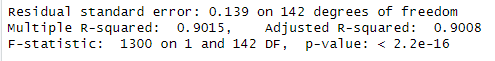
\includegraphics[width=4in]{img/7c.PNG}}}
\notab{\center{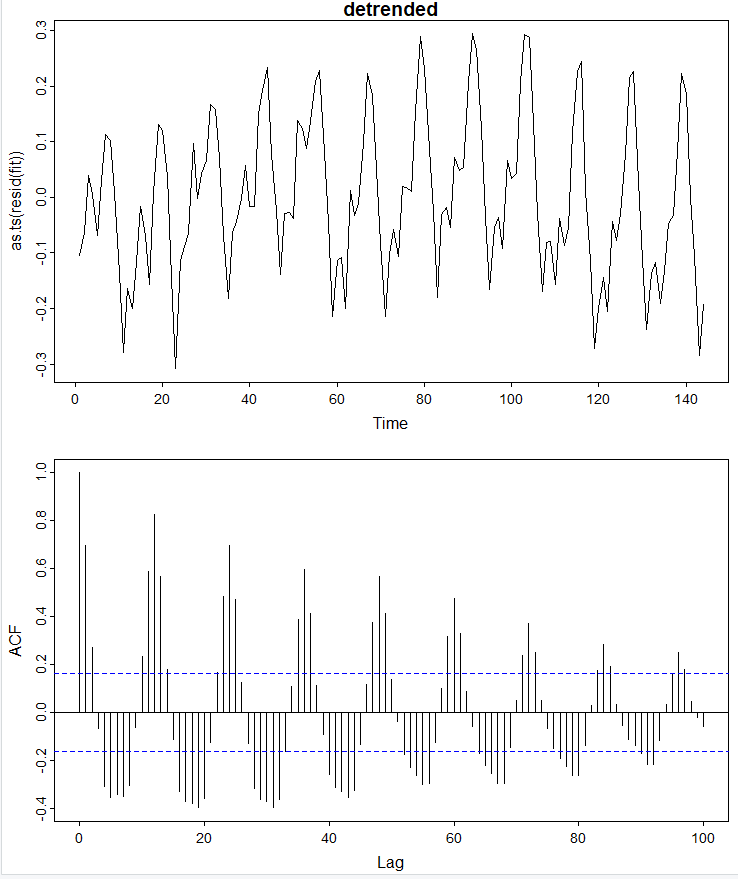
\includegraphics[width=4.5in]{img/7cGraph.PNG}}}

An $R^2 = 0.9$ is a strong linear trend because 90\% of the variance is explained by the model.

\nnl\notab{\textbf{\textit{One can also remove the trend by differencing}}}